%%%%%%%%%%%%%%%%%%%%%%%%%%%%%%%%%%%%%%%%%%%%%%%%%%%%%%%%%%%%%%%%%%%%%%%%%%
% 東京農工大学 工学部 機械システム工学科 中間発表前刷り用スタイルファイル
% Thanks to 佐久間先生 and 佐久間研の皆さん
% 書式設定部分のみ分離&いくつかコマンド定義&微修正 by 本堂
% 2013年度版でテンプレートに変更点があったので修正 by 恒岡
% 2016年度版でテンプレートに変更点があったので修正 by 熊谷
%%%%%%%%%%%%%%%%%%%%%%%%%%%%%%%%%%%%%%%%%%%%%%%%%%%%%%%%%%%%%%%%%%%%%%%%%%
\documentclass[a4paper,twocolumn,twoside,fleqn,leqno,10pt]{jarticle}
\usepackage[dvipdfmx]{graphicx}
\usepackage[dvipdfmx]{color}
\usepackage{bm}
\usepackage{fancyhdr}
%\usepackage{nidanfloat}
\usepackage{float}
%\date{\today 版}\西暦

\usepackage{booktabs}
\usepackage{amsmath}
\usepackage{amssymb}

%微分演算子関係
\newcommand{\dd}{\mathrm{d}} %微分演算子の"d"はローマン体
\newcommand{\diff}[2]{\frac{\mathrm{d}#1}{\mathrm{d}#2}} %常微分
\newcommand{\ddiff}[3]{\frac{\mathrm{d}^#1 #2}{\mathrm{d} #3^#1}} %高階常微分
\newcommand{\pdiff}[2]{\frac{\partial #1}{\partial #2}} %偏微分
\newcommand{\pddiff}[3]{\frac{\partial^#1 #2}{\partial #3^#1}} %高階偏微分

% 以下書式設定(一般) %%%%%%%%%%%%%%%%%%%%%%%%%%%%%%%%%%%%
\setlength{\hoffset}{-5mm}
\setlength{\voffset}{-9mm}
\setlength{\oddsidemargin}{0mm}
\setlength{\evensidemargin}{\oddsidemargin}
\setlength{\topmargin}{0mm}
\setlength{\headheight}{0mm}
\setlength{\headsep}{0mm}
\setlength{\textwidth}{180mm}
\setlength{\textheight}{255mm}
\setlength{\columnsep}{10mm}
\setlength{\topskip}{19.00pt}
\setlength{\mathindent}{4mm}
%\setlength{\kanjiskip}{0.00zw plus.1zw}
\setlength{\kanjiskip}{0.05zw plus.1zw}

\setlength{\floatsep}{3pt plus 1pt minus 1pt}
\setlength{\textfloatsep}{5pt plus 1pt minus 0.5pt}
\setlength{\intextsep}{5pt plus 1pt minus 0.5pt}
\setlength{\dblfloatsep}{3pt plus 1pt minus 1pt}
\setlength{\dbltextfloatsep}{3pt plus 1pt minus 1pt}

\setlength{\parskip}{0pt}
\setlength{\parindent}{1zw}
\setlength{\partopsep}{0pt}

% 英文概要設定 %
\def\abstract{\list{}{\listparindent=1zw \itemindent=\listparindent%
\leftmargin=5mm \rightmargin=\leftmargin}\item[]
\let\endabstract\endlist}

% 脚注の設定 %
\def\thefootnote{}

% 各節タイトル %
\def\thesection {\arabic{section}.}
\def\thesubsection {\arabic{section}$\,\cdot\,$\arabic{subsection}}
\def\thesubsubsection {\thesubsection$\,\cdot\,$\arabic{subsubsection}}

% 数式環境 %
\newdimen\vs % 機械学会書式(added by A.Sakuma)
\def\gyo[#1]{\\ \vbox to#1\vs\bgroup\vss}
\def\endgyo{\vss\egroup\vspace{-1.2mm}}%
\def\LABEL#1{\dotfill\hspace*{9.0mm}\label{#1}}
\def\LABELW#1{\dotfill\hspace*{23.0mm}\label{#1}}
\def\DOTFILL#1{\unitlength=1mm\begin{picture}(#1,3)
 \put(0,0){\makebox(#1,1.5)[b]{\dotfill}}\end{picture}}

% 図の配置設定 %
\def\topfraction{1.0} % 機械学会書式(changed by A.Sakuma)
\setcounter{bottomnumber}{6} % 機械学会書式(changed by A.Sakuma)
\def\bottomfraction{1.0} % 機械学会書式(changed by A.Sakuma)
\setcounter{totalnumber}{8} % 機械学会書式(changed by A.Sakuma)
\def\textfraction{0.0} % 機械学会書式(changed by A.Sakuma)
\def\floatpagefraction{0.7} % 機械学会書式(changed by A.Sakuma)
\setcounter{dbltopnumber}{8}% 機械学会書式(changed by A.Sakuma)
\def\dbltopfraction{1.0} % 機械学会書式(changed by A.Sakuma)
\def\dblfloatpagefraction{0.7} % 機械学会書式(changed by A.Sakuma)
% ```````````````````````````````````````````````````````
% 以下書式設定(特殊) %%%%%%%%%%%%%%%%%%%%%%%%%%%%%%%%%%%%
\makeatletter
% 各節タイトル %
\def\section{\@startsection {section}{1}{0.0ex}{1.62ex}{1.62ex}{\center\rm\bf}}%%セクションを太字に2018諸岡
\def\subsection{\@startsection{subsection}{2}{0.0ex}{1.0ex}{.5ex}{\rm}}%タイトルの後改行
%タイトルを中央揃えにする場合は@startsectionの第6引数を{\center\bf}にする
\def\subsubsection{\@startsection{subsubsection}{3}
{3.0ex}{0.0ex}{-6.0ex}{\rm}}
\def\quote{\list{}{\rightmargin=10mm \leftmargin=\rightmargin}\item[]}%
\long\def\@makecaption#1#2{
\vskip 10pt 
\setbox\@tempboxa\hbox{#1  #2}
\ifdim \wd\@tempboxa >\hsize \settowidth{\labelwidth}{#1} \textwidth=\hsize
\addtolength{\textwidth}{-\labelwidth}\addtolength{\textwidth}{-6pt}
\tabcolsep=2pt\begin{tabular*}{\hsize}{@{\extracolsep{\fill}}lp{\textwidth}}
 #1&\setlength{\baselineskip}{9.0pt}\setlength{\lineskip}{-0.5pt}#2\\
 \end{tabular*}\par\else\hbox to\hsize{\hfil\box\@tempboxa\hfil} \fi}
\def\fnum@figure{\small{Fig.\thefigure}}

% 引用の設定 %
\def\@cite#1#2{$^{\hbox{\scriptsize({#1\if@tempswa , #2\fi})}}$}
\def\thebibliography#1{\section*{{\bf{文  献}}\@mkboth
 {REFERENCES}{REFERENCES}}\list
% {(\hfill\arabic{enumi}\hfill)}{\settowidth\labelwidth{1pt} \leftmargin 30pt
 {(\hfill\arabic{enumi}\hfill)}{\settowidth\labelwidth{1pt} \leftmargin\labelwidth %文献のインデントを左端にした。
 \advance\leftmargin\labelsep
 \usecounter{enumi}}
 \def\newblock{\hskip .11em plus .33em minus .07em}
 \sloppy\clubpenalty4000\widowpenalty4000
 \sfcode`\.=1000\relax}

% 数式環境 %
\def\@eqnnum{\hbox to .01pt{}
 \rlap{\rm \hskip -0.125\displaywidth(\theequation)}}
\def\eqnarray{\stepcounter{equation}\def\@currentlabel{\p@equation\theequation}%
 \global\@eqnswtrue\m@th\global\@eqcnt\z@\tabskip\@centering\let\\\@eqncr
 $$\everycr{}\halign to\displaywidth\bgroup\hskip\@centering$\displaystyle
 \tabskip\z@skip{##}$\@eqnsel&\global\@eqcnt\@ne \hfil$\displaystyle{{}##{}}$\hfil
 &\global\@eqcnt\tw@ $\displaystyle{##}$\hfil\tabskip\@centering
 &\global\@eqcnt\thr@@ \hb@xt@\z@\bgroup\hss##\egroup\tabskip\z@skip\cr}  
\def\@eqnnum{\hbox to .01pt{}%
 \rlap{\rm \hskip -0.10\displaywidth(\theequation)}}
\def\fnum@table{Table \thetable.}
\def\thetable{\@arabic\c@table}

%% Figure 環境中で Table 環境の見出しを表示・カウンタの操作に必
\newcommand{\figcaption}[1]{\def\@captype{figure}\caption{#1}}
\newcommand{\tblcaption}[1]{\def\@captype{table}\caption{#1}}

\makeatother


\usepackage{ifthen}
\newcommand{\secret}[2]{
  \ifthenelse{\equal{#1}{m}}{
    \thispagestyle{fancy}
    \lhead{
      \vspace{-10mm}
      \begin{picture}(0,0)
        \fboxrule=0.5mm
        \hspace{#2}\fcolorbox{red}{white}{{\large {\bf \textcolor{red}{専攻外秘}}}}
    \end{picture}
    }
  }{
    \thispagestyle{fancy}
    \lhead{
      \vspace{-10mm}
      \begin{picture}(0,0)
        \fboxrule=0.5mm
        \hspace{#2}\fcolorbox{red}{white}{{\large {\bf \textcolor{red}{学科外秘}}}}
      \end{picture}
    }
  }
}
\newcommand{\pagenum}[1]{%
\chead{}
\rhead{ \sf{#1} }%%フォントを変更2018諸岡
\lfoot{}
% \cfoot{ \bf{#1} } %ページ数
\cfoot{}
\rfoot{}
}
\renewcommand{\headrulewidth}{0pt}
\renewcommand{\footrulewidth}{0pt}

\pagestyle{empty}
\renewcommand{\title}[2]{
%\twocolumn[%
 \begin{center}
 {\Large\bf #1}\\%日本語タイトルも太字に変更2018諸岡
 {\bf #2}%英語タイトル太字に変更
\end{center}
\vspace{-5mm}
}
\renewcommand{\author}[3]{
 \begin{flushright}
  % \begin{center}
  \begin{small}
    #1\hspace{6mm}#2\hspace{3mm}#3\\
  \end{small}
  % \end{center}
 \end{flushright}
% ]
}
\newcommand{\keyword}[1]{
 \begin{center}{\small
  \begin{tabular*}{150mm}{lp{140mm}}
    \hspace{-17mm}\sl{Key Words} %%Key Word(細字イタリック)に変更2018諸岡
    \rm{: #1}
  \end{tabular*}
 }\end{center}
\vspace{-3mm}
}

%% \newcommand{\keyword}[1]{
%%  \begin{center}{\small
%%   \begin{tabular*}{150mm}{lp{140mm}}
%%   \hspace{-17mm}$\sl{KeyWord}$: &%%Key Word(細字イタリック)に変更2018諸岡
%% #1
%%   \end{tabular*}
%%  }\end{center}
%% \vspace{-3mm}
%% }

%\newenvironment{doctmp}{\begin{document}}{\end{document}}
%\renewenvironment{document}{\begin{doctmp}\begin{small}}{\end{small}\end{doctmp}}
% キーワード
% \begin{center}{\small
 % \begin{tabular*}{138mm}{lp{112mm}}
 % $\mathit{Key Words}$: &
%Upright Posture Control Probrems,
%Agonist, Antagonist, 
%Bio-Motion Controll Problems,
%Muscle, 
%Biological soft tissue 
%Viscoelasticity, 
%2-DOF Robot, 
%  \end{tabular*}
 %}\end{center}
%\vspace{-3mm}
%\setlength{\baselineskip}{4.38mm}    %%% 60行指定(機械科前刷仕様)
%\setlength{\baselineskip}{4.30mm}
%\setlength{\baselineskip}{4.65mm}
\setlength{\vs}{\baselineskip}
\vspace{-\baselineskip}
%\begin{small}
\setlength{\baselineskip}{4.30mm}
%%%%%%%%%%%%%%%%%%%%%%%%%%%%%%%%%%%%%%%%%%%%%%%%%%%%%%%%%%%%%%%%%%%%%%%%%%%%%%

\usepackage{jtygm}
\usepackage{ikuo}
\pagenum{A-17}%ページ番号
\secret{m}{0mm}                 %学外秘/専攻外秘の設定.学部はb(学外秘),修士はm(専攻外秘)にする.
                                %第2引数は位置の調整用.-側に大きくすれば左に寄る.+側に大きくすれば右に寄る.
\newcommand{\FIGDIR}{./fig}	%図を置くディレクトリを指定する
				%Makefileとは連動していないので注意
\setlength{\headheight}{15pt} % 1行目にエラーが出るときは\begin{document}の前にこれを入れると良い
\begin{document}
\twocolumn[%
\title{四肢から独立した仮想翼で羽ばたいて飛ぶ感覚の提示}{Presenting the sensation of flying with flapping virtual wings independent of the limbs}
\author{水内研究室}{遠藤 健}{Ken ENDO}

\begin{abstract}
  % まず日本語版(緒言ではなく要旨)を作る→英訳
  %  ヒトは古くから空を飛ぶことに憧れを抱いている.本研究では,トビトカゲ(天使)のような四肢から独立した翼が背中から生えた生物になり羽ばたいて飛ぶ感覚を提示する方法について提案する.腕を動かして羽ばたいて飛ぶ感覚を提示する研究と異なり,腕を動かさないで羽ばたいて飛ぶ感覚を提示することで,疲労感を軽減し没入感を高めることができる.本稿では,四肢を用いず翼を操作している感覚の提示方法と,VR空間で翼に作用する力をヒトに伝達する手法を提案した.また,被験者実験のために倫理審査を行い実験環境を作成した.
  Since ancient times, people have longed to fly in the sky. In this study, we propose a method of presenting the sensation of flying with flapping virtual wings independent of the limbs, such as the Draco.Unlike studies that present the sensation of flying with flapping wings by moving the arms, this study presents the sensation of flying with flapping wings without moving the arms, which reduces fatigue and increases immersion. In this paper, we proposed a method of presenting the sensation of manipulating the wing without using the limbs and a method of transmitting the force acting on the wing to humans. In addition, an ethical review was conducted and an experimental environment was created for the subject experiment.
  

\end{abstract}

\keyword{anacatestisia(floating feeling), sensation of flying with flapping, virtual wings, EMS, independent of the limbs}
% キーワードもう少し考える
]

\begin{small}
\section{緒  言}
  ヒトは古くから空を飛ぶことに憧れを抱いている.実際に飛ぶことにはリスクが伴うが,VR装置を使用することで簡単に飛行体験が可能である.本研究では,VR装置を用いてトビトカゲのような四肢から独立した翼が背中から生えた生物になり羽ばたいて飛ぶ感覚を提示する手法を提案する.
  
  ヒトに飛ぶ感覚を与える研究において,視覚の変化を与えることによって飛ぶ感覚を与える研究は数多くある.しかし鳥のように羽ばたいて飛ぶ感覚を与える研究は少ない.さらに言えば,トビトカゲのように四肢から独立した翼を持つ生物になり羽ばたいて飛ぶ感覚を与える研究は見当たらない.

  従来は,ヒトが鳥のように腕を動かすことによって羽ばたいて飛ぶ感覚を提示していたがそれによって疲労感が生まれていた.
  四肢を用いず翼を操作している感覚の提示・VR空間で翼に作用する力をヒトに提示する手法を考案し,羽ばたいて飛ぶ感覚を腕を動かさずに提示することで疲労感が減り,VR空間での没入感が増すと考える.


\section{仮想翼の提示と仮想翼で飛ぶ感覚の提示}
  本研究では「羽ばたいて飛ぶ感覚」を「浮遊感」,「飛ぶ感覚」を用いて次のように位置づける.
  「浮遊感」とは,空中に浮いて漂っているような感覚を指す.「飛ぶ感覚」は浮遊感に空中を移動する感覚を追加したものとする.本稿で注目する「羽ばたいて飛ぶ感覚」は,飛ぶ感覚に加え,翼を羽ばたかせる感覚を追加したものである.

  \subsection{仮想翼の提示}
    ヒトは身体像と呼ばれる,自身の身体形状を想像する能力を有している.それにより自己とそれ以外を区別することができる.しかし,自己以外の部分に身体像が拡張する場合がある.身体像の拡張に関する研究についてラバーハンド錯覚についての研究がある\cite{botvinick1998rubber}.目の前にラバーハンドを置きその横に自分の手を並べて仕切り板等で見えなくする.その後,ラバーハンドと自分の手を筆で同時に触ることで,ラバーハンドが自分の手であるかのように感じるという錯覚である.
    
    このように提示される視覚からの情報と,触覚の情報の位置が一致または近しければ身体像を拡張することが可能と考える.本研究では仮想翼の視覚情報と触覚情報の位置を揃えることで,ヒトに仮想翼の提示を行う.  

    % EMSを用いた力覚については後ろで


    % \begin{figure}[b]
    %   \begin{center}
    %     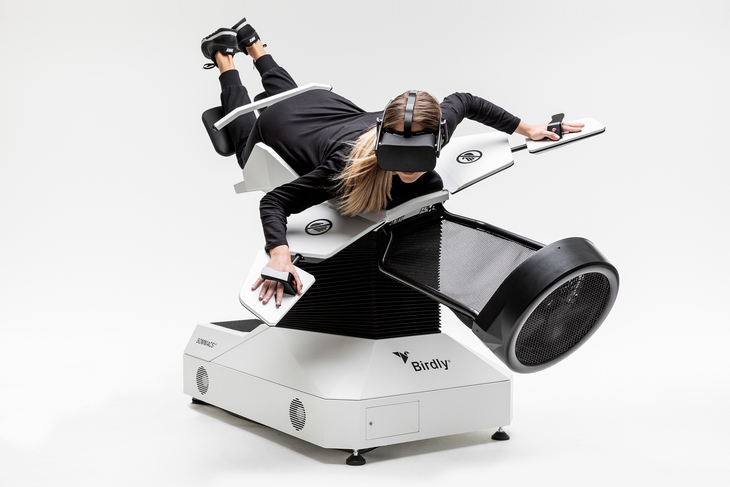
\includegraphics[width=0.60\hsize]{\FIGDIR/Birdly.jpg}%
    %     \caption{Birdly}
    %     \figlabel{Birdly}
    %   \end{center}
    % \end{figure}
  

  \subsection{仮想翼で飛ぶ感覚の提示}


    ベクションと呼ばれる,視野の大部分に一様な運動刺激を提示すると刺激の運動方向と反対の方向に体が動いているように感じる錯覚がある\cite{妹尾武治2014ベクションとその周辺の近年の動向}.例として,停車中の電車から動き出す他の電車の視覚情報を受け取ると,観測者側の電車が動いているように感じる現象が挙げられる.
    浮遊感に関する研究で,ベクションによる落下感覚を分析した研究がある\cite{奥川夏輝2017VR空間における視覚刺激によって発生する落下感覚の分析}.

    また,飛行中の鳥を体験する研究の一例としてBirdly\cite{rheiner2014birdly}がある.操縦装置にうつ伏せで搭乗し手と腕を用いて翼を動かしながら,鳥視点での景色の映像を提示することで,飛行中の鳥のような体験できる装置である.
    しかし,台の上にうつ伏せの体勢になり,腕や手を羽ばたかせるのは不要な疲労感が生まれる.また体の可動域を制限されることは,VR体験の没入感に対し弊害となる.本研究で翼の操作に四肢以外を用いるのは,飛行体験中の疲労感を軽減し没入感を高めるためである.

    % もう一つの例として,上半身のジェスチャーでドローンを操作し飛んでいる感覚を得る?ものがある.こちらは先ほどのものよりも疲労感が多く,外部デバイスも必要である.

    上述したことを踏まえ,本研究ではベクションを用いた浮遊感の提示の手法,疲労感を軽減するために四肢以外を用いた仮想翼の操作の手法を提案する.

  
\section{仮想翼で羽ばたいて飛ぶ感覚の提示方法}
  本研究で提案する,仮想翼で羽ばたいて飛ぶ感覚を提示する方法の概要を\figref{Experimental_method_eng_v2}に示す.
  システムの概要は,「ヒトからデバイスへ情報を送るシステム」と「デバイスからヒトへ情報を送るシステム」の2つに分類した.
  
  \begin{figure}[t]
    \begin{center}
      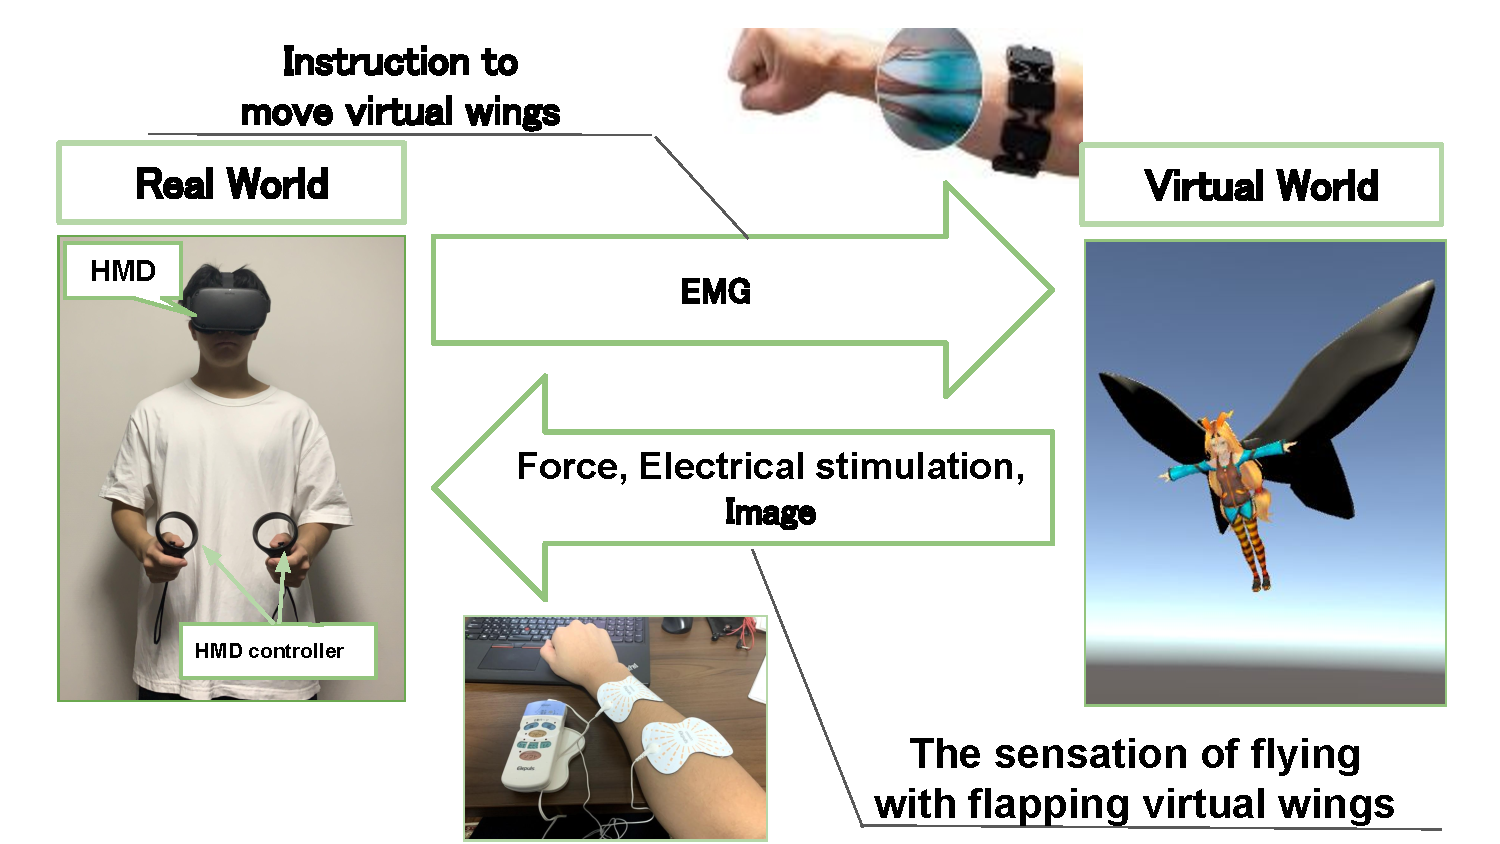
\includegraphics[width=1.00\hsize]{\FIGDIR/Experimental_method_eng_v2}%
      \caption{Research concept}
      \figlabel{Experimental_method_eng_v2}
    \end{center}
  \end{figure}
  % 図のモデルを人形にした方が良い,余計な情報を削除

  \subsection{ヒトからデバイス}
    仮想翼の操作はヒトからデバイスに情報を送るシステムより行う.このシステムは,人体の筋電値を読み取みとりその値によって仮想翼が動作するよ仕様である.\figref{Manipulation_of_virtual_wings_using_Myo_v2ario}に手首の動きに
    合わせて仮想翼の骨組みを動作させた実験の様子を示す.筋電値計測デバイスはMyo(Thalmic labs社),仮想翼の骨組みはUnityを用いて作成した.翼の操作方法は手首を内側に曲げると翼が内側へ曲がり,手首を外側に開くと翼も外側へ開く仕様である.実験より,筋電値による翼の操作の有用性を確認した.また,著者の主観ではあるが3人称視点では仮想翼が自分の背中から生えているという状況を想定しづらいことも確認した.

    \begin{figure}[t]
      \begin{center}
        \vspace{3mm}
        \includegraphics[width=1.00\hsize]{\FIGDIR/Manipulation_of_virtual_wings_using_myo_v2ario.pdf}%
        \caption{Manipulation of virtual wings skeleton using Myo}
        \figlabel{Manipulation_of_virtual_wings_using_Myo_v2ario}
      \end{center}
    \end{figure}
    
    
  \subsection{デバイスからヒト}
    ヒトへ仮想翼を使って羽ばたいて飛ぶ感覚を提示はデバイスからヒトへのシステムより行う.このシステムは,視覚による仮想翼で飛ぶ感覚を提示するシステムと,力覚提示による仮想翼で羽ばたく感覚を提示するシステムの2つに分類する.
    
    視覚による仮想翼で飛ぶ感覚を提示するシステムはヘッドマウントディスプレイ(以後HMD)を用いる.飛ぶ感覚は,飛行体験時の風景の映像よりベクションを促すことで再現する.また,仮想翼の映像より自分の背から翼が生えている感覚を提示する.これにより仮想翼で飛ぶ感覚を再現する.

    力覚提示による仮想翼で羽ばたいて飛ぶ感覚を提示するシステムは,翼のそれぞれの位置に作用する力をヒトへ提示する際,\figref{How2present_force_applied2wings_eng}のように力覚の提示位置をヒトの背中に対応させることで翼がしなる様子を再現する.本研究では力覚の提示方法は2種類検討しいる.1つ目はモータによる振動または押す力を活用したものである.2つ目はEMS(神経筋電気刺激療法)という筋肉や運動神経へ電気刺激を与えることで筋収縮を促し,筋肉の増強や萎縮の予防等をする治療法を活用したものである.この原理を応用し,筋肉を収縮させることで疑似的に重量を知覚させる研究がある\cite{小川剛史2017電気的筋肉刺激が重量知覚に及ぼす影響の分析}.本研究では,EMS機器により筋収縮を起こすことで疑似的に力覚を提示し,使用者に仮想翼に作用する力を提示する.



    \begin{figure}[t]
      \begin{center}
        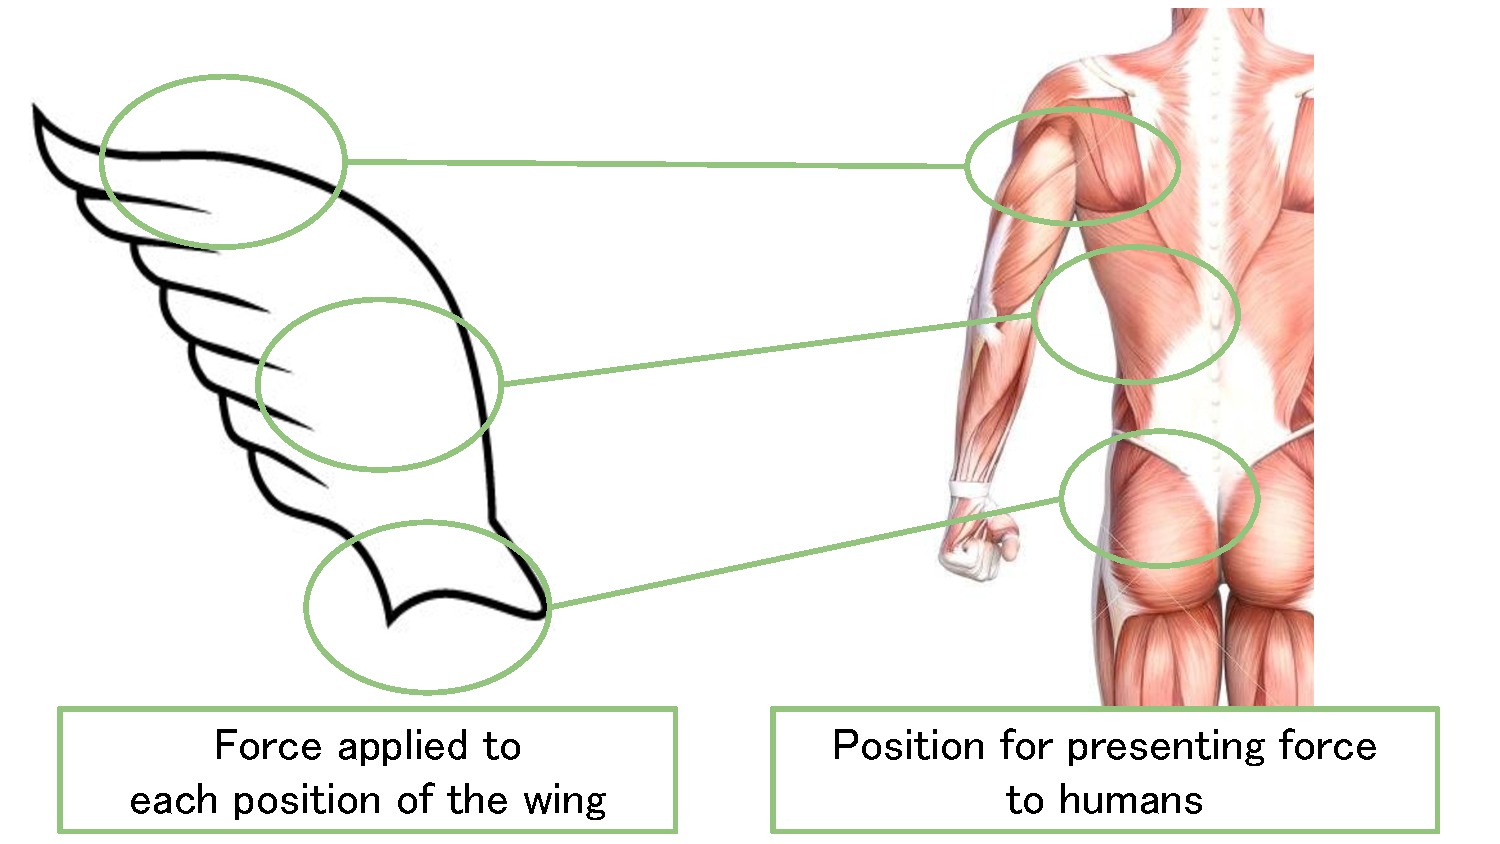
\includegraphics[width=1.00\hsize]{\FIGDIR/How2present_force_applied2wings_eng.pdf}%
        \caption{How to present force applied virtual wings}
        \figlabel{How2present_force_applied2wings_eng}
      \end{center}
    \end{figure}



\section{被験者実験}
  % 実験の目的→方法の順番で書くこと
  被験者実験では,筋電計測位置と羽ばたく感覚の提示位置を変化させた場合の没入感の違いについて検証する.
    
  被験者はHMD,筋電計測装置,羽ばたく感覚の提示装置を装着し,仮想翼を操縦する.この際,被験者の筋電のデータを記録する.
  筋電計測装置に関してはMyoWare(Advancer Technologies)を使用し体に直接貼り付けて計測を行う.筋電取得位置は関節動作を伴わない静的な筋収縮が容易な部位である胸肩部・腹部・臀部を検討している.
  羽ばたく感覚の提示に関しては,ハプティックスーツによる振動・押す力,またはEMS機器の筋収縮作用による疑似的な力覚提示によって行う.羽ばたく感覚提示の位置に関しては仮想翼が存在する背中から体の側面を検討している.
  
  その後,操縦中の没入感に関して被験者の回答を得る.被験者へは筋電取得箇所と力覚提示提示位置ごと没入感の違いについての回答を得る.具体的には以下のような内容を検討している.
  \begin{itemize}
    \item 筋電計測位置別の没入感
    \item 力覚提示位置別の没入感
    \item ハプティックスーツとEMS機器の没入感
    \item 没入感において筋電計測位置の羽ばたく感覚の提示位置重要性の比較
    \item どの組み合わせが一番没入感が高かったか
  \end{itemize}
  % 質問の意図に関しては記載する必要があるのだろうか.(スペース的に省略しても良いのだろうか)
    

  % --------以下倫理審査の書類を参考にして作成--------------
  % 倫理審査,コロナ関係は1段落で簡潔に触れる程度とする
  本実験は「東京農工大学 人を対象とする研究に関する倫理審査委員会の倫理審査」を通過しており,実験は被験者の同意を得て行う.
  % 被験者の募集は学内メーリングリスト, 掲示, アルバイト募集用WEBサイトなどを利用して行う. 被験者の選定方針に関しては特に定めない.ただし, 未成年の場合には保護者の承諾を取ることとする. 
  また,被験者に生じるリスクとしては,実験中に発生するVR酔いや新型コロナウイルス感染症への感染がある.これらのリスクは,感染症予防対策を十分に行い,被験者が体調に違和感を感じたらすぐに対応することで対策をする.
  
  % 被験者実験の様子(予定)の図があるともっとわかりやすいかも



\section{結言}
  本稿では,翼を動かして飛ぶ感覚を与える研究に注目し,四肢を用いず翼を操作している感覚の提示方法と,VR空間で翼に作用する力をヒトに伝達する手法を提案した.また,被験者実験のために倫理審査を行い実験環境を作成した.

  今後の予定として,筋電計測位置・羽ばたく感覚の提示位置を変化させた場合の没入感の違いについて検証するために被験者実験を行う.その結果から得られる最も評価が高い筋電計測位置・羽ばたく感覚の提示位置より,没入感が高いシステムを作成する.また,デバイスからヒトへの提示情報として前庭電気刺激による加速度感覚\cite{青山一真2014前庭電気刺激における逆方向不感電流を用いた加速度感覚の増強}の追加も検討している.

 % 少なくとも1つは参考文献をciteしないとエラーが起きる

{
\small
 \setlength{\kanjiskip}{0.0zw plus.01zw} %
 \setlength{\baselineskip}{9pt}        %
 \setlength{\itemsep}{0.2pt}             %
 \setlength{\lineskip}{0pt}              %
%% \scriptsize %%←どうしても入らない時は,このコメントをはずすと少し小さくなる.
\bibliographystyle{junsrt}
\bibliography{reference}
}



%% \end{thebibliography}
\end{small}
\end{document}
